% Options for packages loaded elsewhere
\PassOptionsToPackage{unicode}{hyperref}
\PassOptionsToPackage{hyphens}{url}
%
\documentclass[
  10pt,
  a4paper]{article}
\title{Analysis 1B --- Tutorial 6}
\author{Christian Jones: University of Bath}
\date{March 2023}

\usepackage{amsmath,amssymb}
\usepackage{lmodern}
\usepackage{iftex}
\ifPDFTeX
  \usepackage[T1]{fontenc}
  \usepackage[utf8]{inputenc}
  \usepackage{textcomp} % provide euro and other symbols
\else % if luatex or xetex
  \usepackage{unicode-math}
  \defaultfontfeatures{Scale=MatchLowercase}
  \defaultfontfeatures[\rmfamily]{Ligatures=TeX,Scale=1}
\fi
% Use upquote if available, for straight quotes in verbatim environments
\IfFileExists{upquote.sty}{\usepackage{upquote}}{}
\IfFileExists{microtype.sty}{% use microtype if available
  \usepackage[]{microtype}
  \UseMicrotypeSet[protrusion]{basicmath} % disable protrusion for tt fonts
}{}
\makeatletter
\@ifundefined{KOMAClassName}{% if non-KOMA class
  \IfFileExists{parskip.sty}{%
    \usepackage{parskip}
  }{% else
    \setlength{\parindent}{0pt}
    \setlength{\parskip}{6pt plus 2pt minus 1pt}}
}{% if KOMA class
  \KOMAoptions{parskip=half}}
\makeatother
\usepackage{xcolor}
\IfFileExists{xurl.sty}{\usepackage{xurl}}{} % add URL line breaks if available
\IfFileExists{bookmark.sty}{\usepackage{bookmark}}{\usepackage{hyperref}}
\hypersetup{
  pdftitle={Analysis 1B --- Tutorial 6},
  pdfauthor={Christian Jones: University of Bath},
  hidelinks,
  pdfcreator={LaTeX via pandoc}}
\urlstyle{same} % disable monospaced font for URLs
\usepackage[margin=2.5cm]{geometry}
\usepackage{longtable,booktabs,array}
\usepackage{calc} % for calculating minipage widths
% Correct order of tables after \paragraph or \subparagraph
\usepackage{etoolbox}
\makeatletter
\patchcmd\longtable{\par}{\if@noskipsec\mbox{}\fi\par}{}{}
\makeatother
% Allow footnotes in longtable head/foot
\IfFileExists{footnotehyper.sty}{\usepackage{footnotehyper}}{\usepackage{footnote}}
\makesavenoteenv{longtable}
\usepackage{graphicx}
\makeatletter
\def\maxwidth{\ifdim\Gin@nat@width>\linewidth\linewidth\else\Gin@nat@width\fi}
\def\maxheight{\ifdim\Gin@nat@height>\textheight\textheight\else\Gin@nat@height\fi}
\makeatother
% Scale images if necessary, so that they will not overflow the page
% margins by default, and it is still possible to overwrite the defaults
% using explicit options in \includegraphics[width, height, ...]{}
\setkeys{Gin}{width=\maxwidth,height=\maxheight,keepaspectratio}
% Set default figure placement to htbp
\makeatletter
\def\fps@figure{htbp}
\makeatother
\setlength{\emergencystretch}{3em} % prevent overfull lines
\providecommand{\tightlist}{%
  \setlength{\itemsep}{0pt}\setlength{\parskip}{0pt}}
\setcounter{secnumdepth}{5}
\newcommand{\BOO}{BOO}
\usepackage {hyperref}
\hypersetup {colorlinks = true, linkcolor = blue, urlcolor = blue}
\usepackage{float}
\ifLuaTeX
  \usepackage{selnolig}  % disable illegal ligatures
\fi

\usepackage{amsthm}
\theoremstyle{plain}
\newtheorem*{theorem*}{Theorem}\newtheorem{theorem}{Theorem}[section]
\theoremstyle{definition}
\newtheorem*{definition*}{Definition}\newtheorem{definition}{Definition}[section]
\theoremstyle{plain}
\newtheorem*{proposition*}{Proposition}\newtheorem{proposition}[theorem]{Proposition}
\newtheorem*{Definitions*}{Definitions}\newtheorem{Definitions}[definition]{Definitions}
\theoremstyle{plain}
\newtheorem*{lemma*}{Lemma}\newtheorem{lemma}{Lemma}[section]
\theoremstyle{plain}
\newtheorem*{corollary*}{Corollary}\newtheorem{corollary}{Corollary}[section]
\theoremstyle{plain}
\newtheorem*{conjecture*}{Conjecture}\newtheorem{conjecture}{Conjecture}[section]
\theoremstyle{definition}
\newtheorem*{example*}{Example}\newtheorem{example}{Example}[section]
\theoremstyle{definition}
\newtheorem*{exercise*}{Exercise}\newtheorem{exercise}{Exercise}[section]
\newtheorem*{Thought*}{Thought}\newtheorem{Thought}{Thought}[section]
\theoremstyle{remark}
\newtheorem*{remark*}{Remark}
\newtheorem*{solution*}{Solution}
\newtheorem*{Example*}{Example}
\theoremstyle{remark}
\newtheorem*{Proof*}{Proof}
\newtheorem*{Examples*}{Examples}
\let\BeginKnitrBlock\begin \let\EndKnitrBlock\end
\begin{document}
\maketitle

{
\setcounter{tocdepth}{2}
\tableofcontents
}
\newpage
\pagenumbering{arabic}

\hypertarget{introduction}{%
\section*{Introduction}\label{introduction}}
\addcontentsline{toc}{section}{Introduction}

Here is the material to accompany the 6th Analysis 1B Tutorial on the 13th March. Alternative formats can be downloaded by clicking the download icon at the top of the page. Please send any comments or corrections to \href{mailto:caj50@bath.ac.uk}{Christian Jones (caj50)}. To return to the homepage, click \href{http://caj50.github.io/tutoring.html}{here}.

\hypertarget{lecture-recap}{%
\section{Lecture Recap}\label{lecture-recap}}

This week, we're starting to look at the derivative of a function. Along the way, we'll see some tricks for making differentiation easier, and we'll cover a way of finding the derivative of inverse functions.

\hypertarget{differentiation}{%
\subsection{Differentiation}\label{differentiation}}

While functions are very good at describing physical quantities such as temperature, density or momentum we can usually gain more insight into these variables by studying how fast they change at a given position or time. Mathematically, we study rates of change using derivatives, which again relies on the ideas behind limits!

\BeginKnitrBlock{definition}[Derivative]
{\label{def:def1} }Let \(f: D \to \mathbb{R}\), where \(D \subseteq \mathbb{R}\) is an open set, and let \(c \in D\). Then, if \(\exists L \in \mathbb{R}\) such that \[\lim_{h \to 0}\frac{f(c+h) - f(c)}{h} = L,\] we say that \(f\) is differentiable at \(c\), and call \(L\) the derivative of \(f\) at \(c\).
\EndKnitrBlock{definition}
We can note a few things here:

\begin{itemize}
\tightlist
\item
  Firstly, if this \(L\) exists, we write it as \(f'(c)\) to make it clear that its a derivative.
\item
  We require \(D\) to be open, so that we can actually take limits! If, for example, \(D = [-1,2]\), we could attempt to define the derivative at any point in the interior of \(D\), \(D^{\circ} = (-1,2)\), but we couldn't define the derivative at \(x = -1\) or \(x = 2\).\footnote{There is nothing stopping us; however, trying to define \emph{left} and \emph{right derivatives} at these points, i.e.~we could search for \[\lim_{x \to -1^{+}}\frac{f(-1+h) - f(-1)}{h}\;\;\text{or}\;\;\lim_{x \to 2^{-}}\frac{f(2+h) - f(2)}{h}.\]}
\item
  Substituting \(x = c+h\) into the definition gives us an equivalent formulation: \(f\) is differentiable at \(c\) if there exists \(L\in\mathbb{R}\) such that \[\lim_{x \to c}\frac{f(x) - f(c)}{x - c} = L.\]
\end{itemize}

One quick result we obtain from this definition is the following:
\BeginKnitrBlock{proposition}
{\label{prp:prop1} }If a function \(f:D \to \mathbb{R}\) is differentiable at a point \(c\), then it is continuous at \(c\).
\EndKnitrBlock{proposition}
The contrapositive of this is very useful for ruling functions out: if a function is \textbf{not} continuous, it is not differentiable. As a further remark, or warning, \textbf{continuity does not imply differentiability}! To see this, think of either \(f(x) = \lvert x \rvert\) at \(x = 0\), or look up the \href{https://en.wikipedia.org/wiki/Weierstrass_function}{Weierstrass function}.

\hypertarget{diff}{%
\subsection{Rules of Differentiation}\label{diff}}

Since everything inside the limit defining the derivative is just a function (of either \(h\) or \(x\)), we can apply the algebra of limits to deduce a few familiar rules of differentiation:

\BeginKnitrBlock{theorem}[Algebra of Derivatives 1]
{\label{thm:thm1a} }Let \(D\subseteq\mathbb{R}\) be an open set, and let \(f,g:D \to \mathbb{R}\) be differentiable at \(c\in D.\) Then the following functions are differentiable at \(c\):

\begin{enumerate}
\def\labelenumi{\arabic{enumi}.}
\tightlist
\item
  \(f+g\), with \[(f+g)'(c) = f'(c) + g'(c),\]
\item
  \(Kf\) for any \(K\in\mathbb{R}\), with \[(Kf)'(c) = Kf'(c),\]
\end{enumerate}
\EndKnitrBlock{theorem}

Using these two rules we can show that the set of functions \(f:D\to\mathbb{R}\) which are differentiable at \(c\) form a vector space. In fact, since differentiability implies continuity, and the zero function \(0:D \to \mathbb{R}\) given by \(0(x) = 0\) is also differentiable at \(c\), this set forms a vector subspace of the set of functions \(f:D \to \mathbb{R}\) which are continuous at \(c\).

There are three further rules which make up the Algebra of Derivatives:

\BeginKnitrBlock{theorem}[Algebra of Derivatives 2]
{\label{thm:thm1b} }Let \(D\subseteq\mathbb{R}\) be an open set, and let \(f,g:D \to \mathbb{R}\) be differentiable at \(c\in D.\) Then the following functions are differentiable at \(c\):

\begin{enumerate}
\def\labelenumi{\arabic{enumi}.}
\setcounter{enumi}{2}
\tightlist
\item
  (Product rule) \(fg\), with \[(fg)'(c) = f'(c)g(c) + f(c)g'(c),\]
\item
  For \(g(c)\neq0\), \(1/g\), with \[\left(\frac{1}{g}\right)'(c) = \frac{-g'(c)}{g(c)^2}.\]
\item
  (Quotient rule) For \(g(c)\neq0\), \(f/g\) with \[\left(\frac{f}{g}\right)'(c) = \frac{f'(c)g(c)-f(c)g'(c)}{g(c)^2}.\]
\end{enumerate}
\EndKnitrBlock{theorem}

One thing to note here is that we can obtain the quotient rule by applying the product rule to the functions \(f\) and \(1/g\), which saves you having to learn the proof!

\hypertarget{chain-rule}{%
\subsubsection{Chain Rule}\label{chain-rule}}

The one thing we've said nothing about so far is whether a composition of functions is differentiable. This result is what is known as the (familiar) chain rule:

\BeginKnitrBlock{theorem}[Chain Rule]
{\label{thm:thm2} }Let \(g:(a,b) \to \mathbb{R}\) and \(f:(A,B) \to \mathbb{R}\) be such that \(g\left((a,b)\right) \subseteq (A,B).\) Assume that \(g\) is differentiable at \(c\) and \(f\) is differentiable at \(g(c)\). Then the composition \(f\circ g\) is differentiable at \(c\) with \[\left(f\circ g\right)'(c) = f'\left(g(c)\right)g'(c).\]
\EndKnitrBlock{theorem}

\hypertarget{inverse-functions}{%
\subsection{Inverse Functions}\label{inverse-functions}}

Another thing we might want to know is whether we can differentiate the inverse of a differentiable function. For example, the exponential function \(\exp\) and the trigonometric functions \(\sin, \cos\) have nice series definitions, and this makes it fairly straightforward to calculate their derivatives. But what if we're interested in their inverses (\(\ln, \arcsin, \arccos\))? Luckily, we have a theorem which tells us what the values of their derivatives are!

\BeginKnitrBlock{theorem}[Inverse Function Theorem]
{\label{thm:thm3} }Let \(f: (a,b) \to (A, B)\) be bijective, and let \(c \in (a,b).\) Assume that \(f\) is differentiable at \(c\), \(f'(c) \neq 0\), and \(f^{-1}\) is continuous at \(f(c).\) Then \(f^{-1}\) is differentiable at \(y_0 = f(c)\) and \[\left(f^{-1}\right)'(y_0) = \frac{1}{f'\left(f^{-1}(y_0)\right)} = \frac{1}{f'(c)}.\]
\EndKnitrBlock{theorem}

\BeginKnitrBlock{example}
{\label{exm:ex1} }Returning to our exponential example from last week, we know that from lectures \(\exp: \mathbb{R} \to (0,\infty)\) is differentiable for all \(c \in \mathbb{R}\), and since \(\exp'(x) = \exp(x)\), \(\exp'(c) \neq 0\) for any \(c\). Last week, we showed that the inverse function \(\ln: (0,\infty) \to \mathbb{R}\) is continuous at any \(\exp(c) \in (0,\infty)\), so by Theorem \ref{thm:thm3}, \(\ln\) is differentiable on \((0,\infty)\), with \[\ln'(y_0) = \frac{1}{\exp'(\ln(y_0))} = \frac{1}{\exp(\ln(y_0))} = \frac{1}{y_0}.\] Graphically, we can see the result of this theorem by comparing the gradient of the associated tangent lines of \(\exp\) and \(\ln\) at the points \((c,\exp(c))\) and \((\exp(c),c)\) respectively. In the graph below, we have taken \(c = 1\) for illustrative purposes.

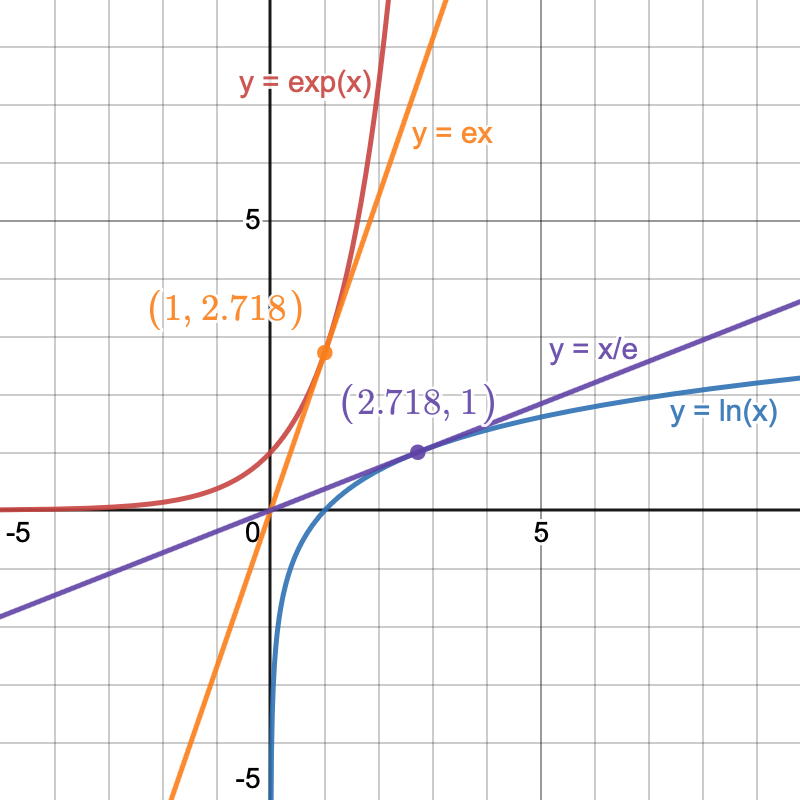
\includegraphics[width=0.3\textwidth,height=\textheight]{./explog2.png}
\EndKnitrBlock{example}

We can use the results of Example \ref{exm:ex1} and the rules of differentiation from Section \ref{diff} to calculate the derivatives of some more complicated functions:
\BeginKnitrBlock{example}
{\label{exm:ex2} }Consider the function \(h:(0,\infty) \to (0,\infty)\) given by \(h(x) = x^x.\) Since \[h(x) = \exp(\ln(x^x)) = \exp(x\ln(x)),\] we can rewrite \(h\) as a composition of differentiable functions \(h = f \circ g\), where \(f:\mathbb{R} \to (0,\infty)\) is defined by \(f(x) = \exp(x)\), and \(g: (0,\infty) \to \mathbb{R}\) is defined by \(g(x) = x\ln(x).\)

From lectures, we know that \(f\) is differentiable on \(\mathbb{R}\) with \(f'(x) = \exp(x).\) Furthermore, by Example \ref{exm:ex1} and the product rule, we know that \(g\) is differentiable on \((0,\infty)\), with \(g'(x) = \ln(x) + 1.\) Hence, by the chain rule, \(h\) is differentiable on \((0,\infty)\) with \[h'(x) = f'(g(x))g'(x) = \exp(x\ln(x))\left(\ln(x) + 1\right) = x^x\left(\ln(x) + 1\right)\]
\EndKnitrBlock{example}

Theorem \ref{thm:thm3} will come in handy if you ever need to perform coordinate transforms, in particular when evaluating integrals by substitution. You may have also come across the multivariate version of this theorem in MA10230 (Multivariable Calculus and Differential Equations) when calculating the Jacobian for a transformation from Cartesian to polar coordinates (or vice versa).

\hypertarget{hints}{%
\section{Hints}\label{hints}}

As per usual, here's where you'll find the problem sheet hints!

\begin{enumerate}
\def\labelenumi{\arabic{enumi})}
\tightlist
\item
  We did some examples similar to this in the tutorial today. Specify the domain of each function, and use the results you've seen in the course to justify differentiability on each domain. In regards to computing the derivatives, I don't think you'll have too much trouble, but let me know if you run into problems.
\item
  The following formula may come in handy:\[\max(f(x),g(x)) = \frac{1}{2}\left(\lvert f(x) - g(x) \rvert + f(x) + g(x)\right).\]
  For the function examples, try and find \(f,g\) such that \[\max(f(x),g(x)) = \lvert x \rvert.\]
\item
  Using \(p(x) = (x-a)q(x)\), what does \(p'(x)\) give you?
\end{enumerate}

\end{document}
